\subsection{Scalar Field} \label{subsec:scalar_field}
The first step in the terrain generation is to generate a scalar field which is a function that takes a point in 3D space and returns a value.
What is important is that this function always returns the same value for the same point.
Another important property is that the function should return close values for close points.
Our function returns values for points that have integer coordinates.

Having these properties in mind we decided to use the Perlin noise function.
Perlin noise first introduced by Ken Perlin in 1983 \cite{Perlin-Noise} is often used in computer graphics and in particular in procedural terrain generation.
It is a pseudo-random function that returns values for any point in 3D space.
\question{Should we explain how the Perlin noise function works? Our implementation does not add anything to it.}
However, unlike some random functions, it returns similar values for similar points.
This makes it ideal for this game.

The Perlin noise function is used to generate a value for each point in the scalar field.
This value is then modified based on 5 parameters: octaves, initial frequency, frequency multiplier, initial amplitude and amplitude multiplier.
How these parameters affect the terrain can be seen in \autoref{fig:argument_comparison}.
These parameters are generated based on the seed of the world from 5 different sets of options which gives the game 5 terrains.
However, we need more than just the value for each point and a normal vector.
Each point is also assigned a type based on the position that is later used to determine the type of the block which in turn determines its color.

\newpage
\begin{figure}[h]
    \centering
    \begin{subfigure}{0.45\textwidth}
        \centering
        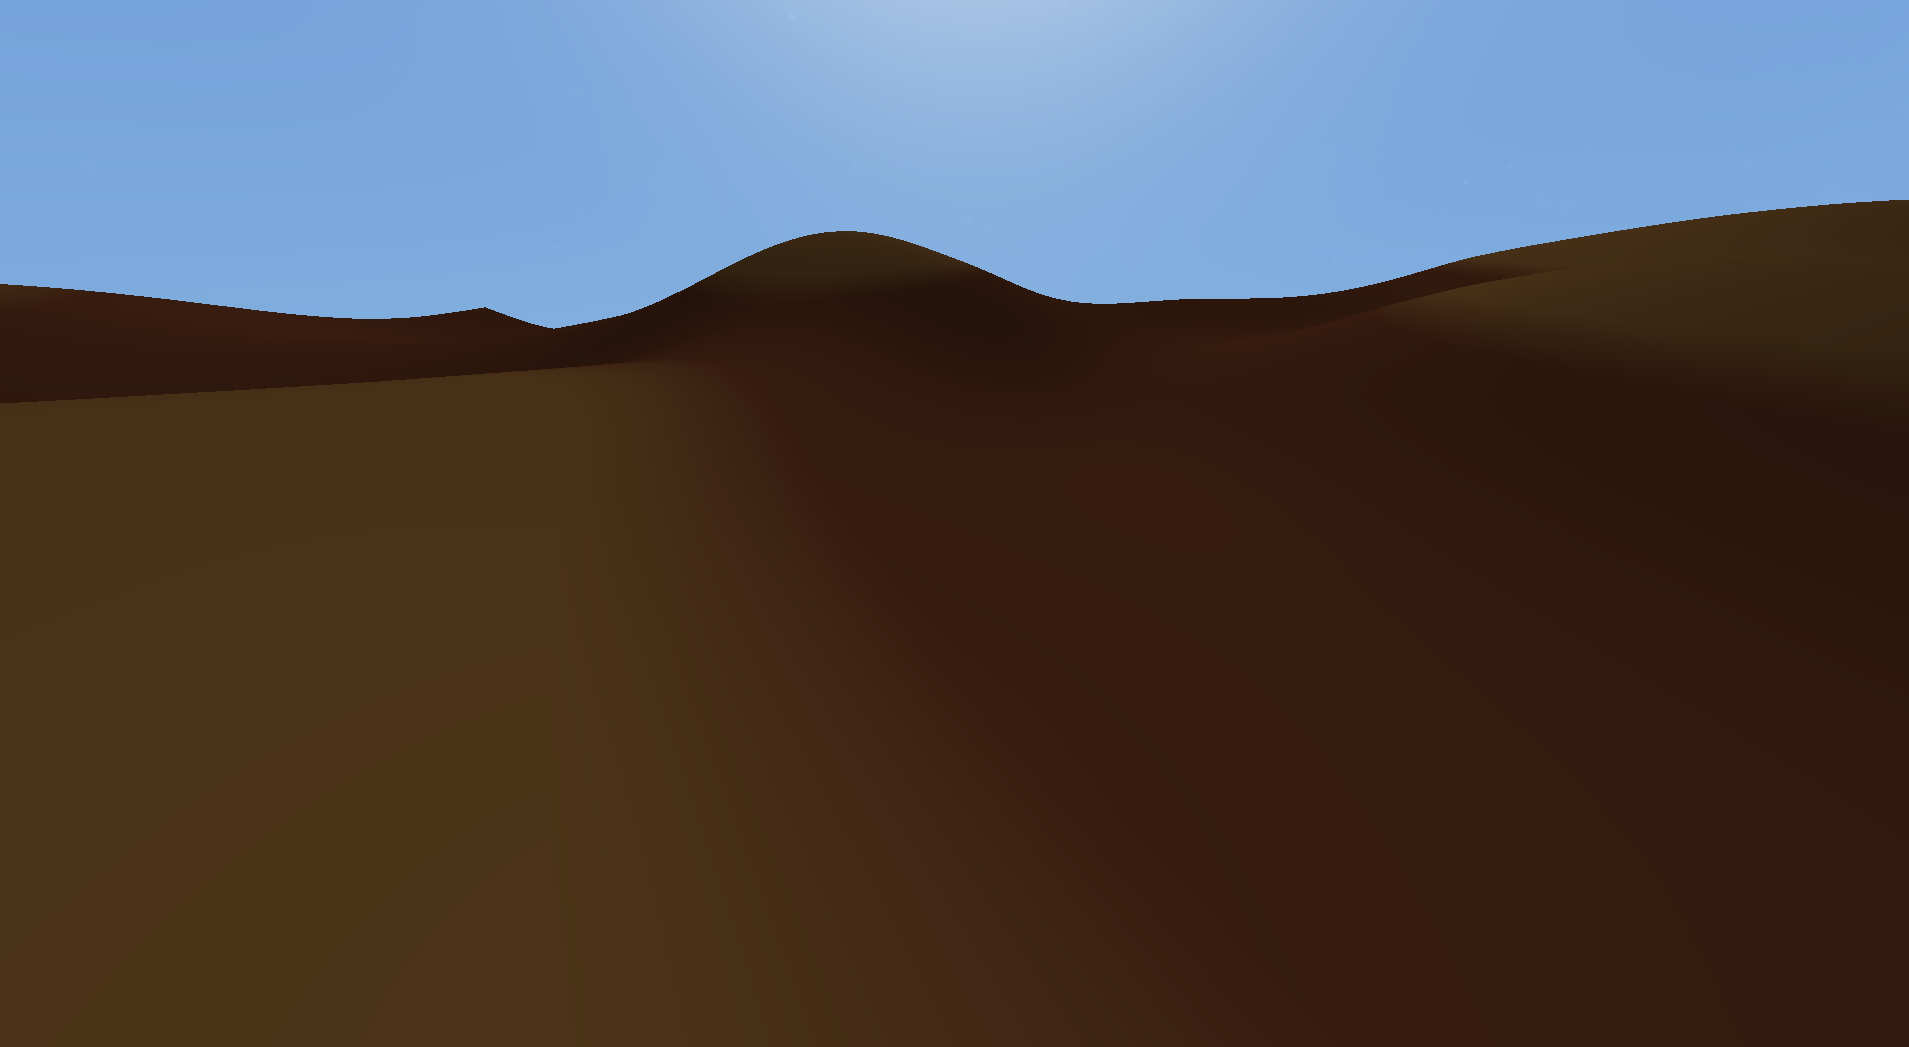
\includegraphics[width=0.8\textwidth]{chapters/system_architecture/sections/terrain/resources/octaves-1.png}
        \caption{Small octaves (1).}
    \end{subfigure}
    \hfill
    \begin{subfigure}{0.45\textwidth}
        \centering
        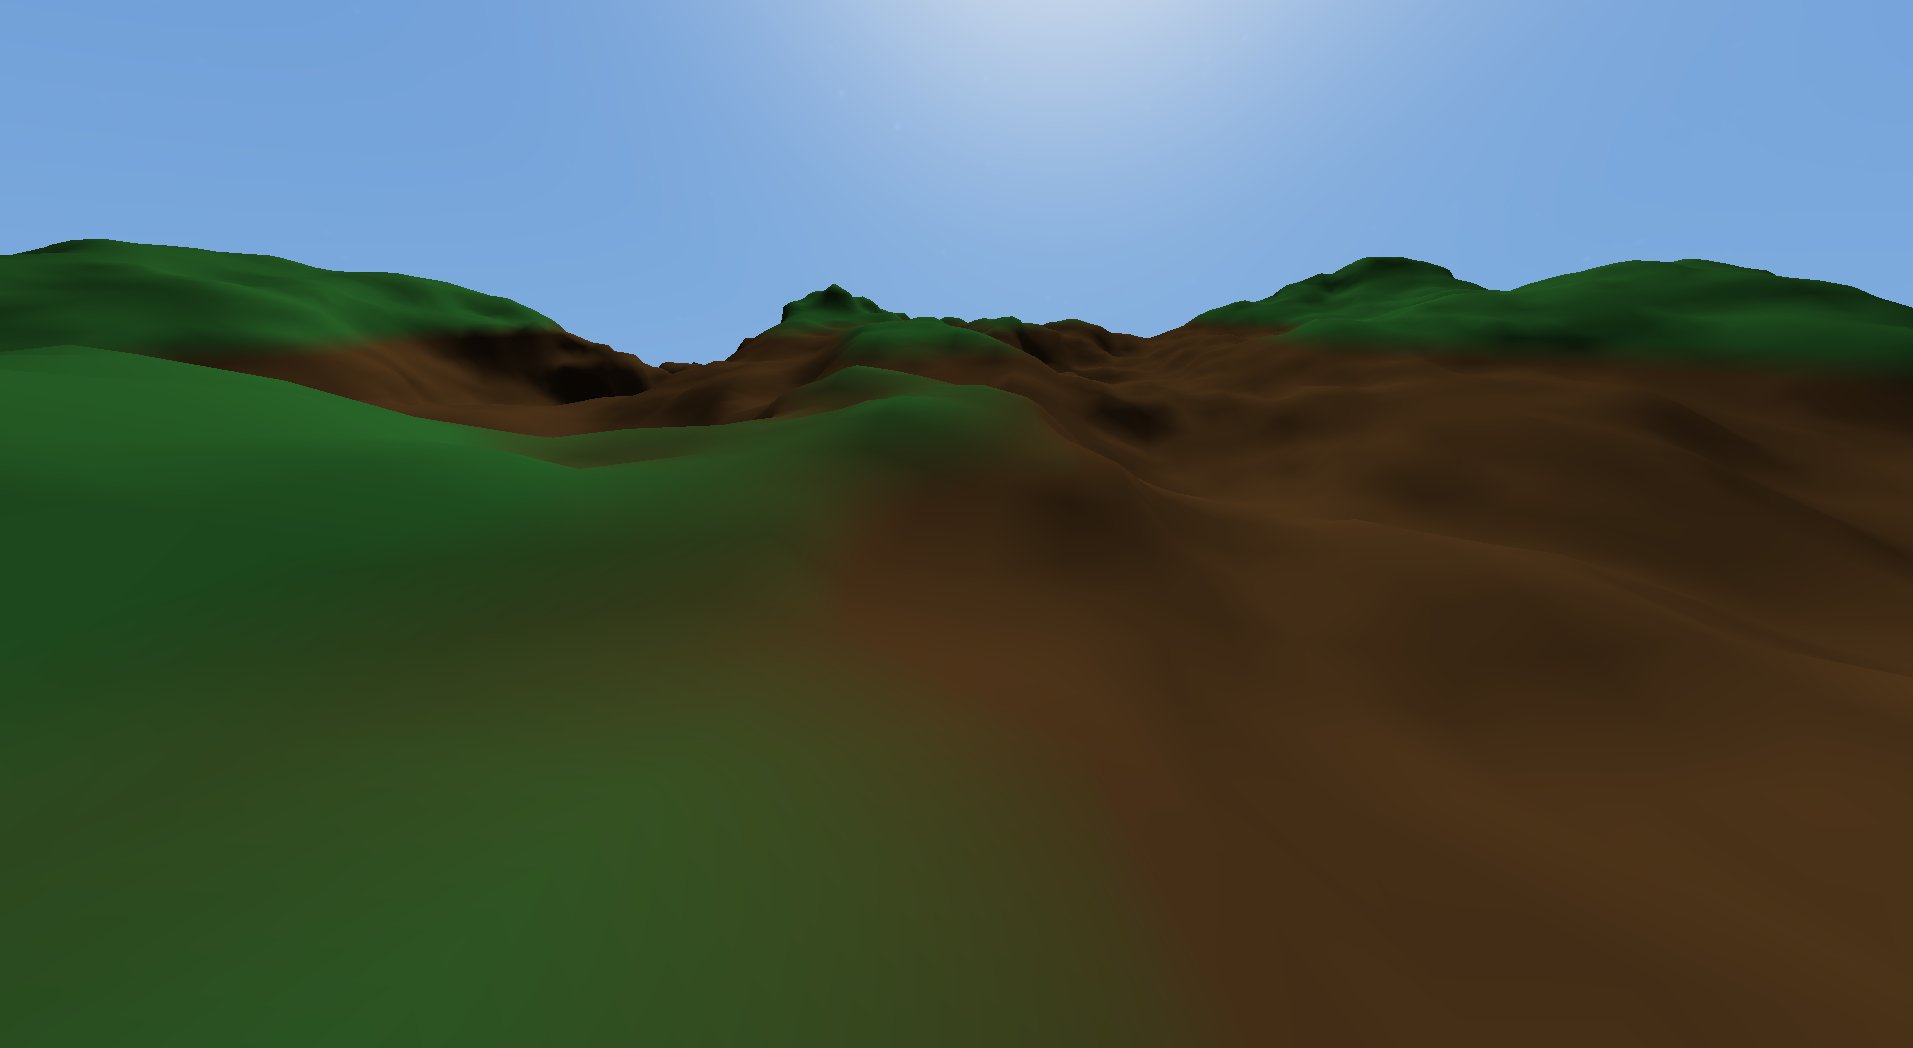
\includegraphics[width=0.8\textwidth]{chapters/system_architecture/sections/terrain/resources/octaves-5.png}
        \caption{Big octaves (5).}
    \end{subfigure}

    \centering
    \begin{subfigure}{0.45\textwidth}
        \centering
        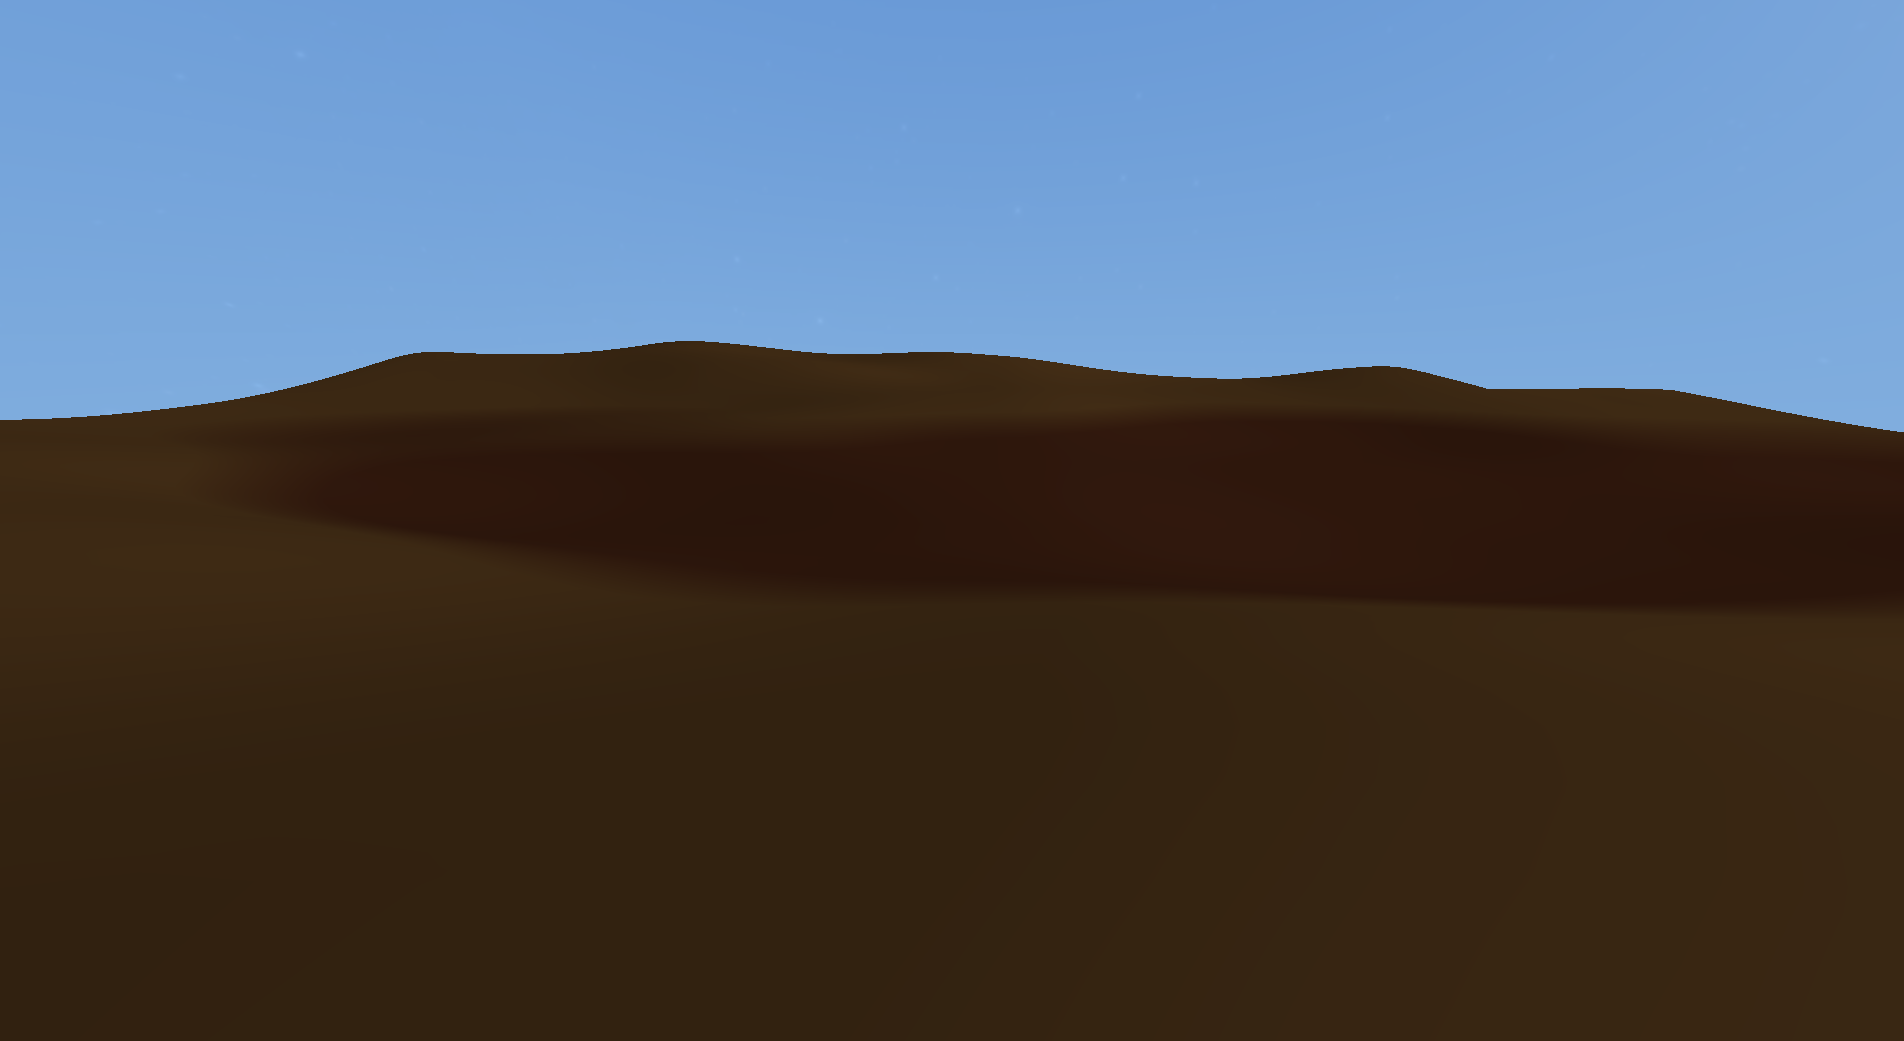
\includegraphics[width=0.8\textwidth]{chapters/system_architecture/sections/terrain/resources/initial-freq-0.1.png}
        \caption{Small initial frequency (1).}
    \end{subfigure}
    \hfill
    \begin{subfigure}{0.45\textwidth}
        \centering
        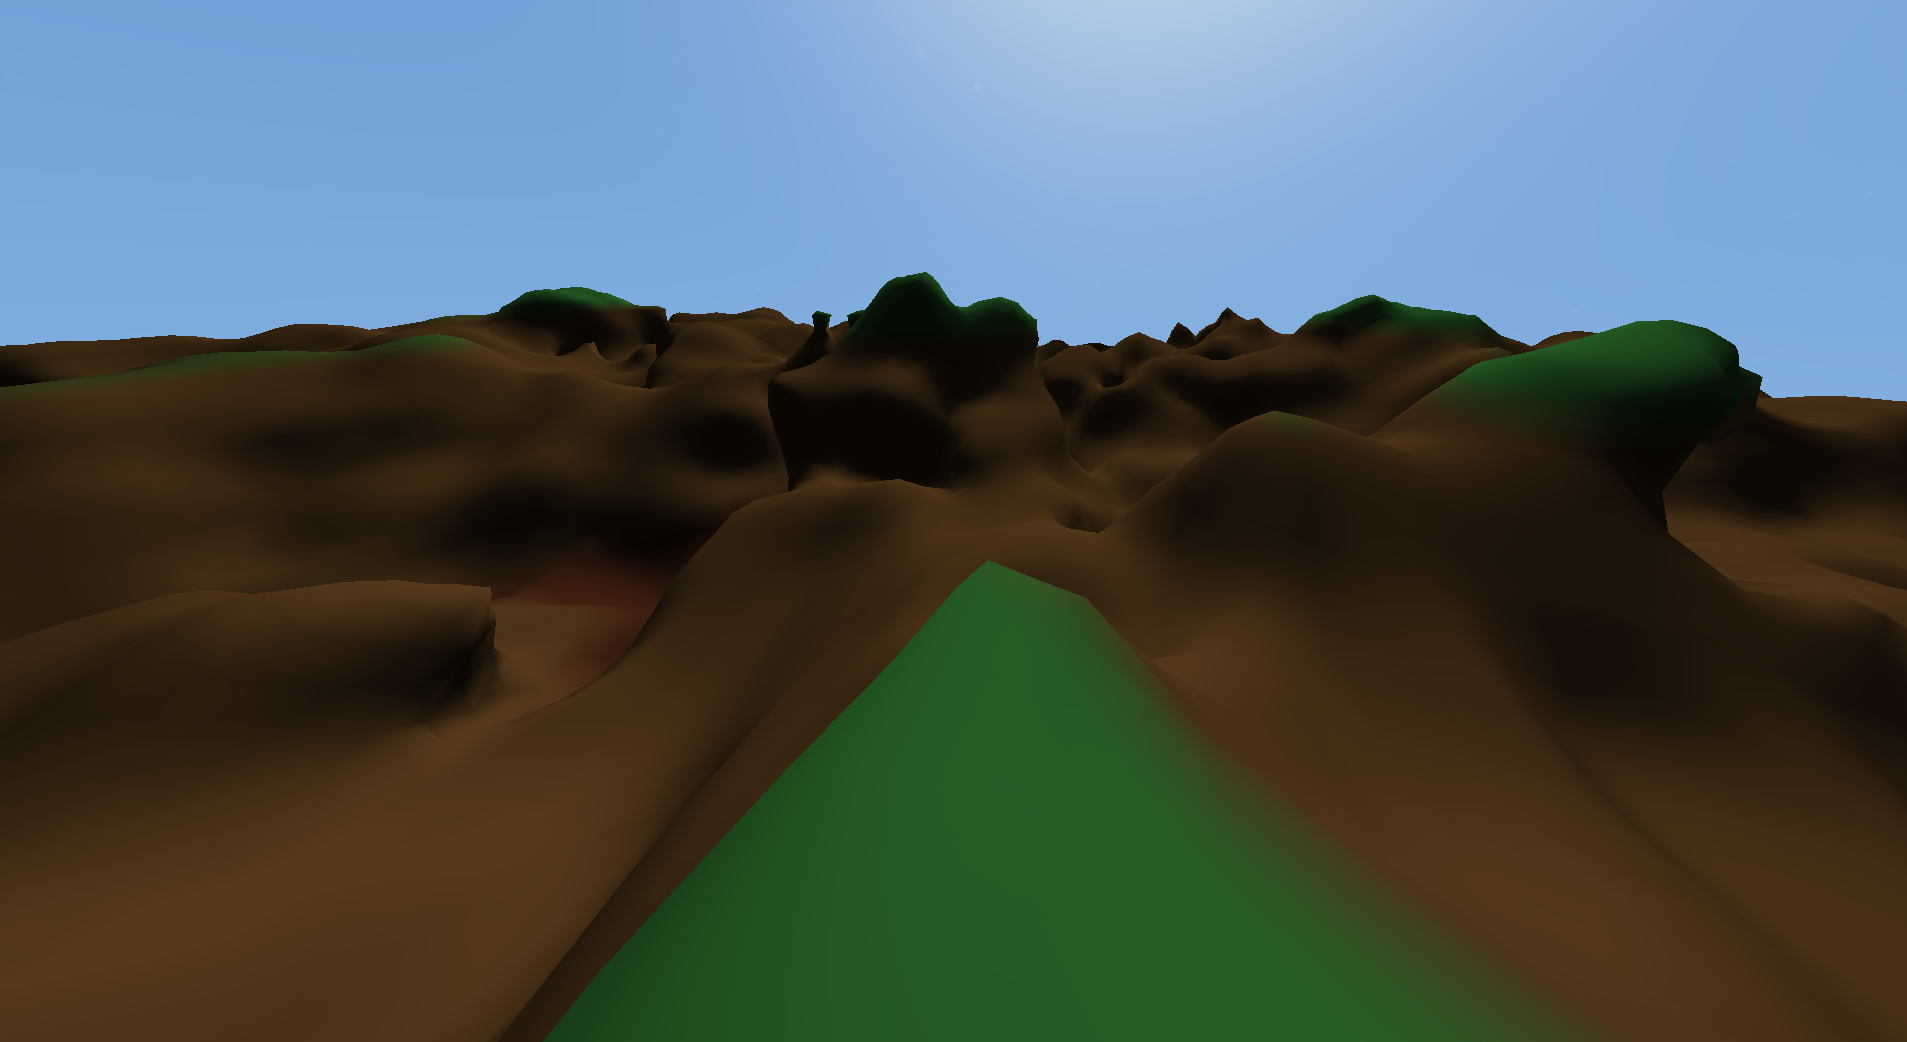
\includegraphics[width=0.8\textwidth]{chapters/system_architecture/sections/terrain/resources/initial-freq-0.5.png}
        \caption{Big initial frequency (0.5).}
    \end{subfigure}

    \centering
    \begin{subfigure}{0.45\textwidth}
        \centering
        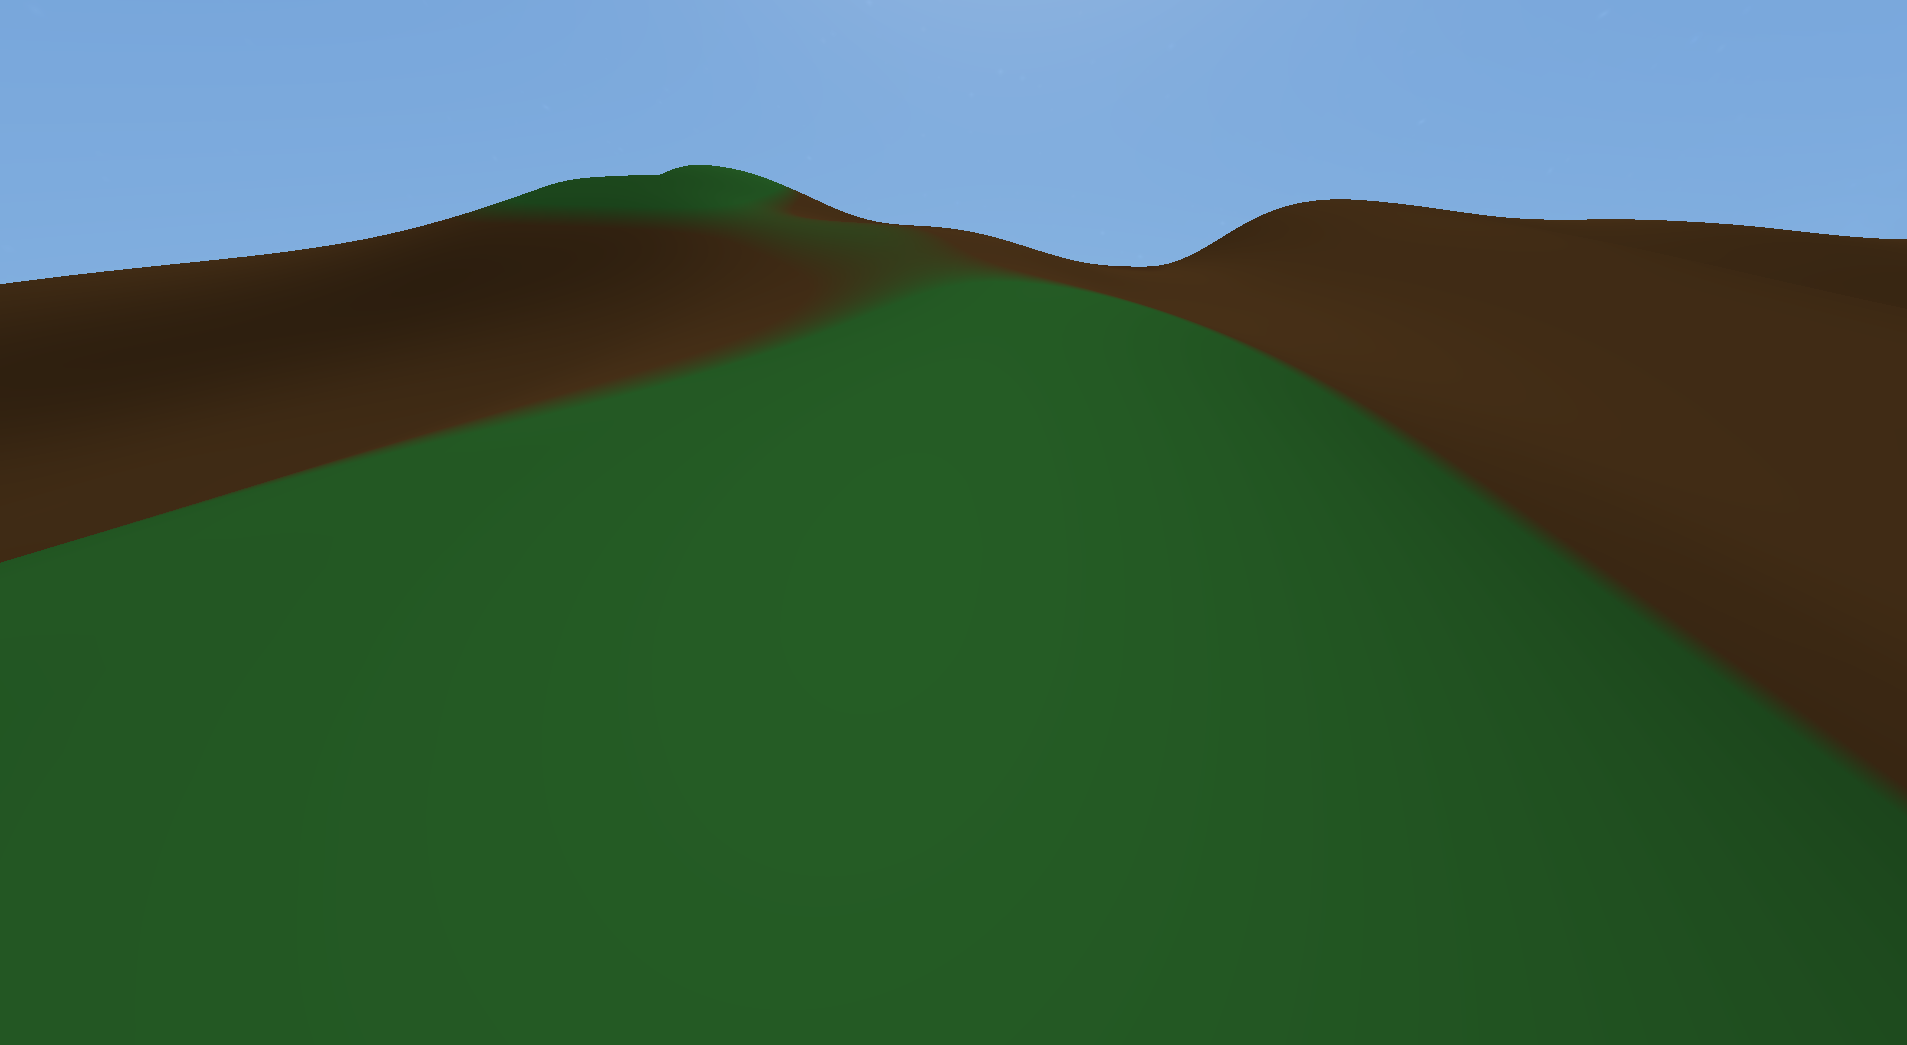
\includegraphics[width=0.8\textwidth]{chapters/system_architecture/sections/terrain/resources/freq-mul-0.5.png}
        \caption{Small frequency multiplier (0.5).}
    \end{subfigure}
    \hfill
    \begin{subfigure}{0.45\textwidth}
        \centering
        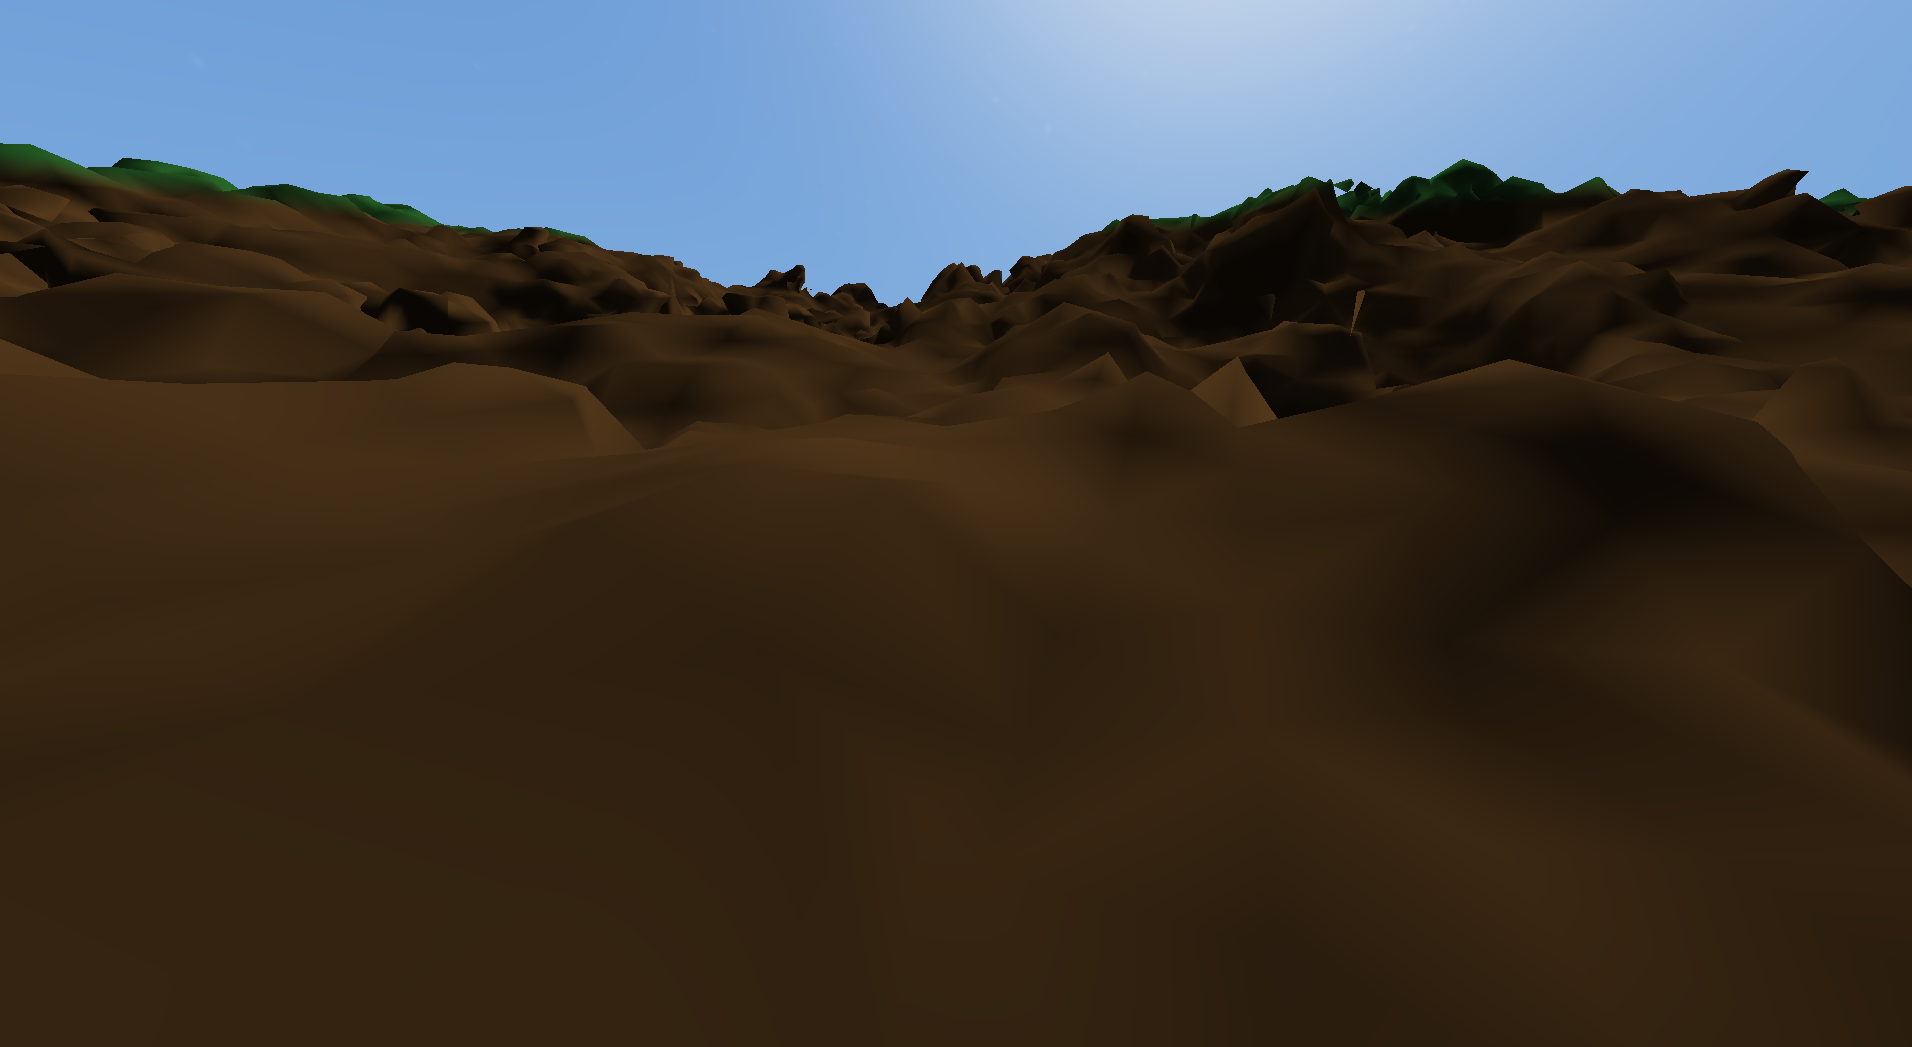
\includegraphics[width=0.8\textwidth]{chapters/system_architecture/sections/terrain/resources/freq-mul-5.png}
        \caption{Big frequency multiplier (5).}
    \end{subfigure}

    \centering
    \begin{subfigure}{0.45\textwidth}
        \centering
        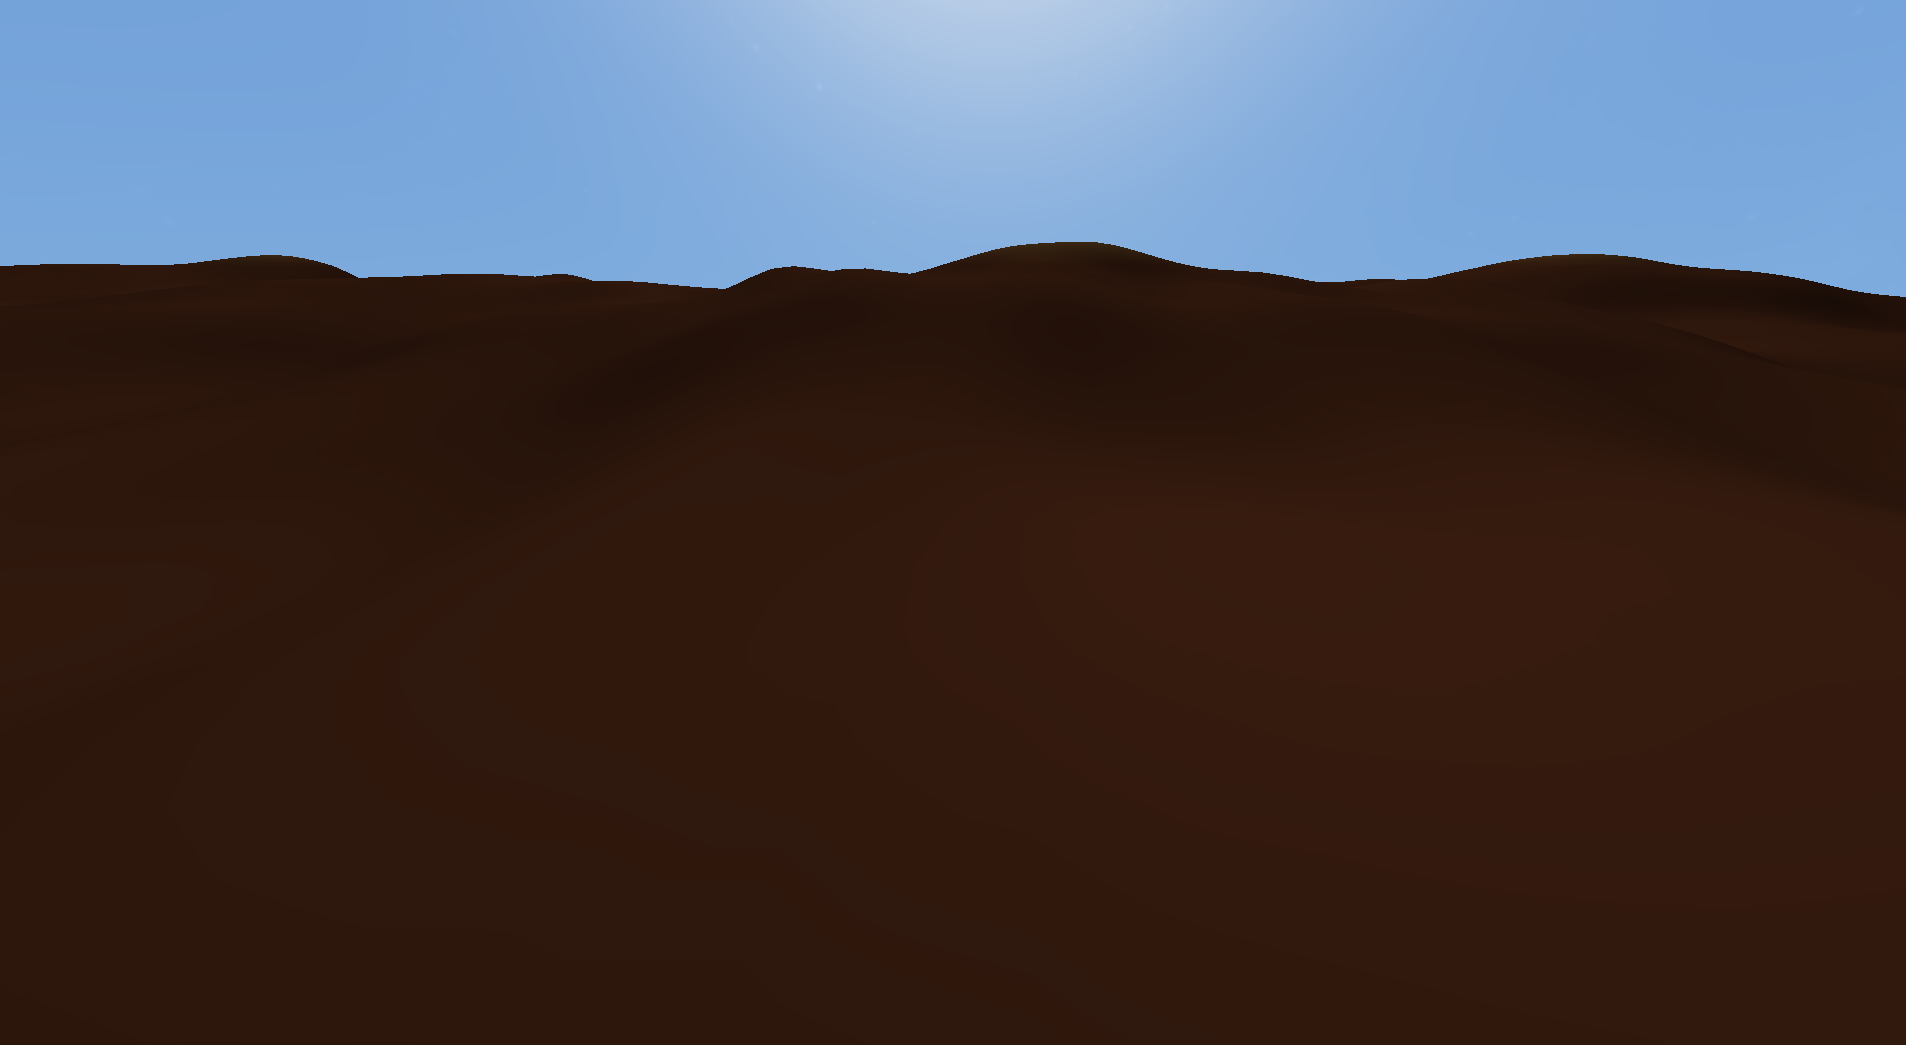
\includegraphics[width=0.8\textwidth]{chapters/system_architecture/sections/terrain/resources/initial-amp-8.png}
        \caption{Small initial amplitude (8).}
    \end{subfigure}
    \hfill
    \begin{subfigure}{0.45\textwidth}
        \centering
        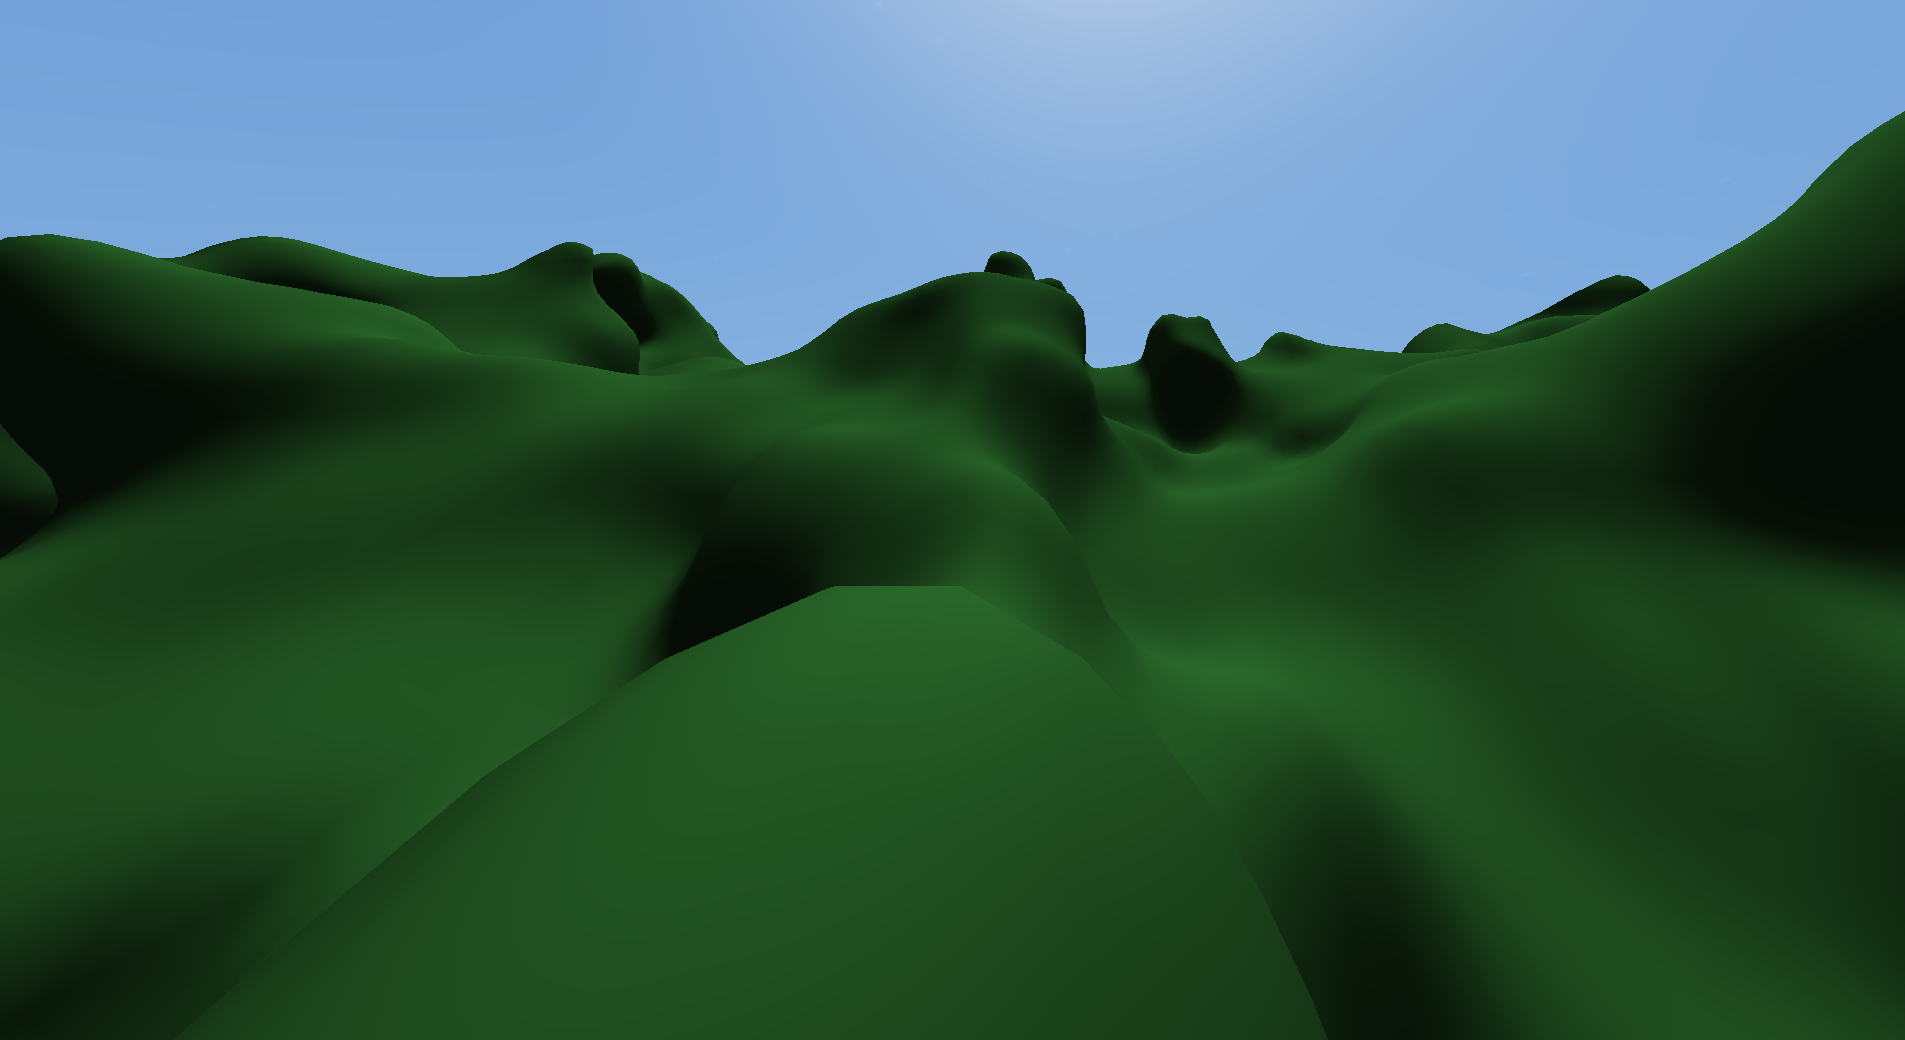
\includegraphics[width=0.8\textwidth]{chapters/system_architecture/sections/terrain/resources/initial-amp-32.png}
        \caption{Big initial amplitude (32).}
    \end{subfigure}

    \centering
    \begin{subfigure}{0.45\textwidth}
        \centering
        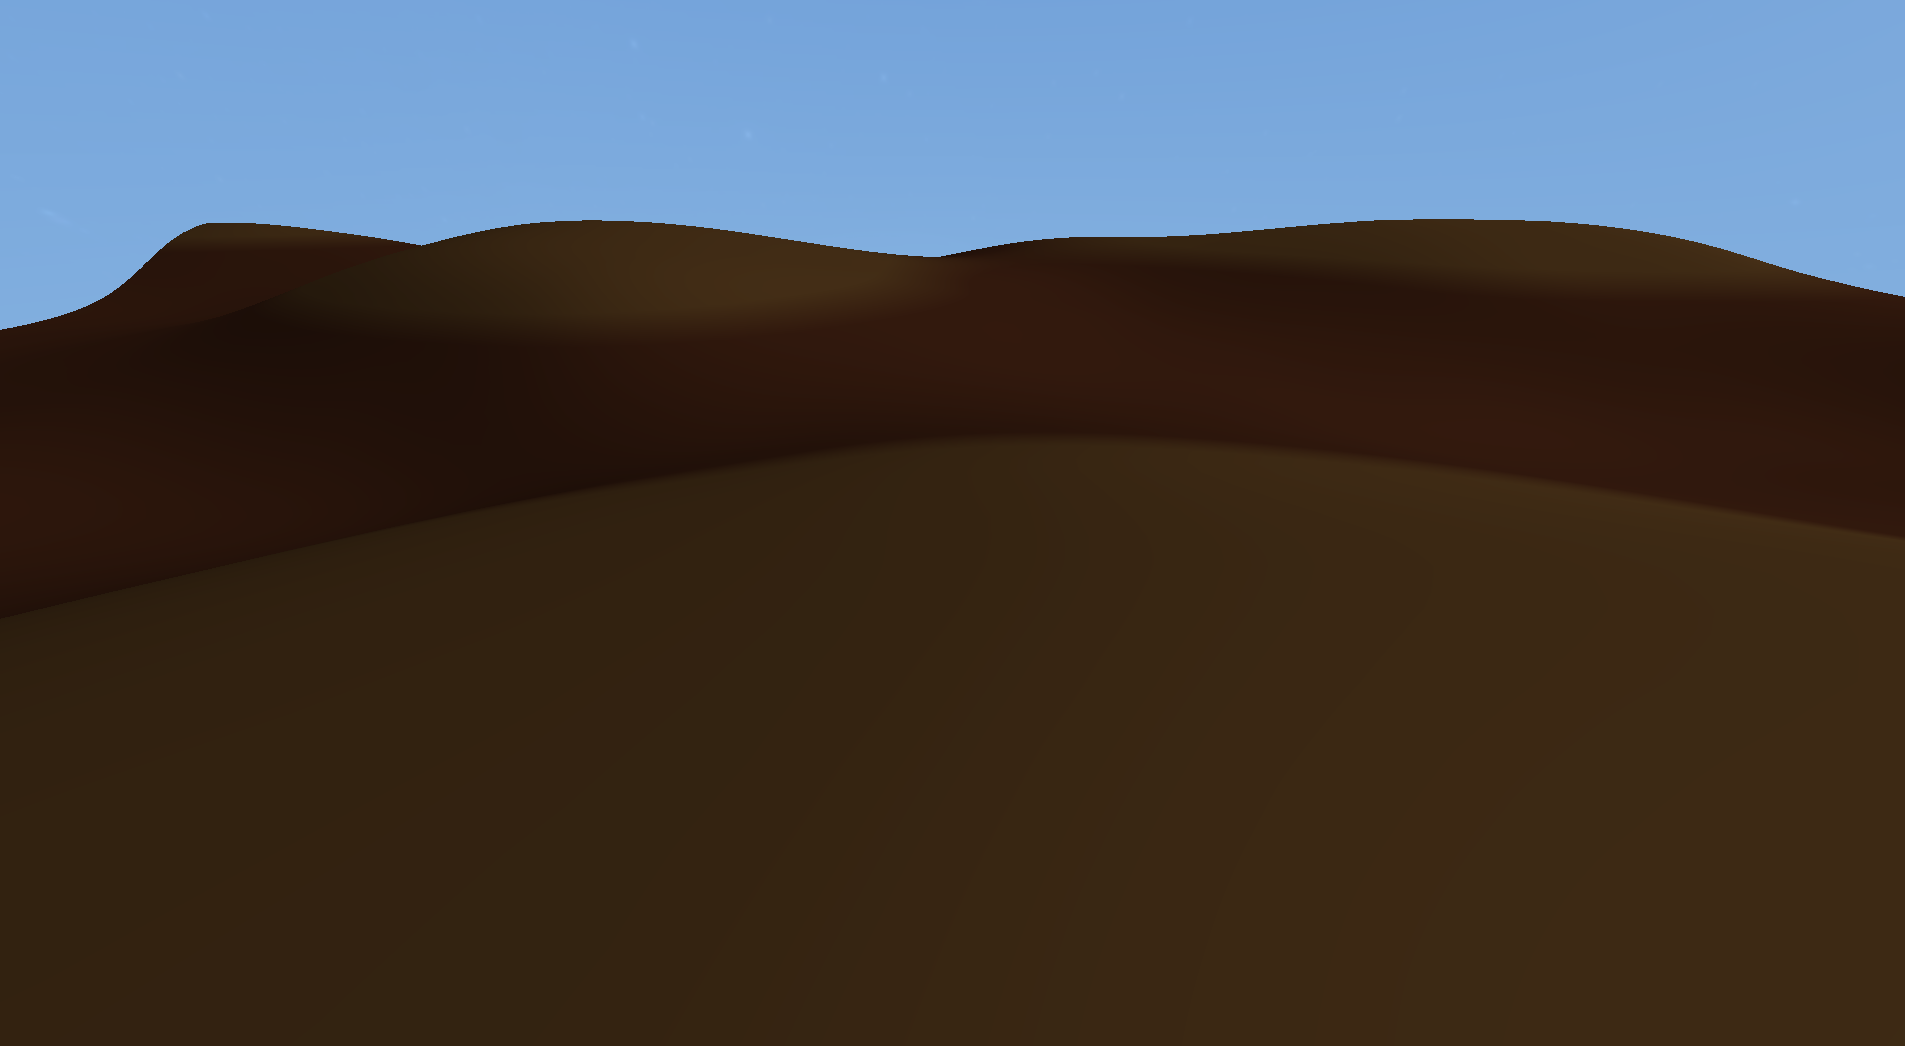
\includegraphics[width=0.8\textwidth]{chapters/system_architecture/sections/terrain/resources/amp-mul-0.1.png}
        \caption{Small amplitude multiplier (0.1).}
    \end{subfigure}
    \hfill
    \begin{subfigure}{0.45\textwidth}
        \centering
        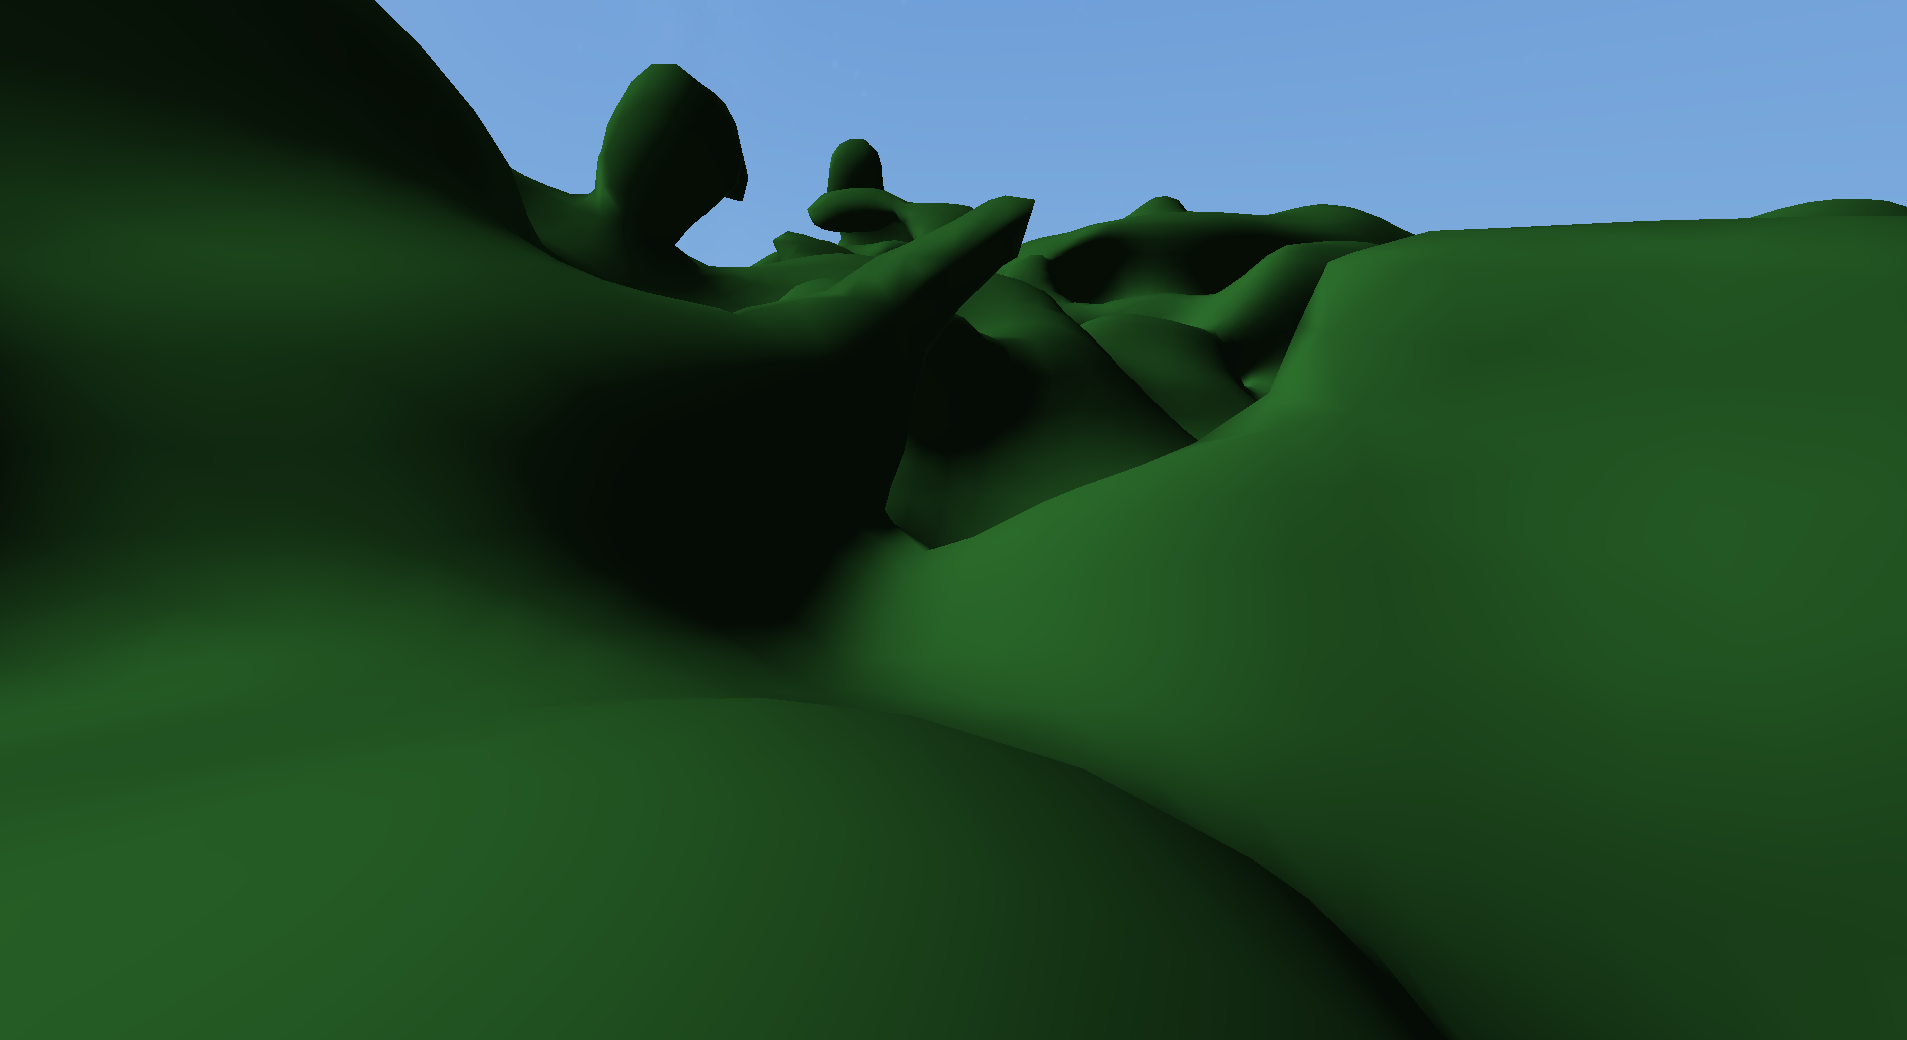
\includegraphics[width=0.8\textwidth]{chapters/system_architecture/sections/terrain/resources/amp-mul-1.png}
        \caption{Big amplitude multiplier (1).}
    \end{subfigure}

    \caption{Scalar field parameter comparison.}
    \label{fig:argument_comparison}
\end{figure}